\chapter{METODOLOGIA}
\label{chp:methodology}
\graphicspath{ {./resources/images/metodologia} }

O objetivo do presente estudo é comparar modelos de \textit{embeddings} para recuperação de código-fonte a partir de buscas feitas em linguagem natural. Para tanto, propõe-se um sistema para a comparação de \textit{embeddings} gerados por \textit{encoders} tanto de linguagem natural quanto de código-fonte.
O presente estudo propõe um sistema, apresentado na figura \ref{fig:metodology-system_overview}, que servirá para comparar modelos de \textit{embeddings} para recuperação de código-fonte a partir de buscas feitas em linguagem natural.

\begin{figure}[htbp]
    \centering
        \caption{Visão geral do sistema}
        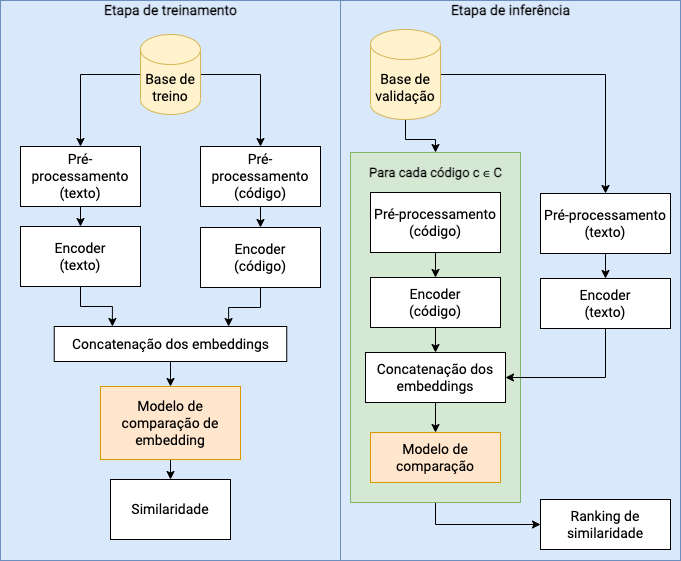
\includegraphics[scale=0.5]{system-overview.png}
        \smallcaption{Fonte: Autor}
        \label{fig:metodology-system_overview}
\end{figure}

\section{Base de Dados}
Todos os experimentos serão realizados utilizando os dados disponibilizados na pela \textit{Microsoft} através do repositório \textit{CodeSearchNet} \cite{Husain2019CodeSearchNetCE}. Esse repositório consiste em uma coleção de bases de dados e métricas voltadas ao problema de busca de código usando linguagem natural.

Para os experimentos do estudo em questão, será utilizada a base de dados principal dessa coleção. Tal base contém dois milhões de pares código-fonte/comentário, vindos de bibliotecas de código aberto. Desses pares existentes na base, os comentários são textos, escritos em inglês, que descrevem o código-fonte correspondente. O código-fonte, por sua vez, são trechos de código-fonte que realizam determinada tarefa. Além disso, nessa base pode-se encontrar pares com código-fonte das linguagens de programação \textit{Python}, \textit{Javascript}, \textit{Ruby}, \textit{Go}, \textit{Java} e \textit{PHP}. Neste trabalho, serão selecionados os pares código-fonte/comentário das linguagens \textit{Java} e \textit{Python}. Essas duas linguagens foram escolhidas por suas diferenças no sistema de tipagem: a primeira é fortemente tipada, enquanto a segunda é fracamente tipada. 

\section{Pré-processamento}
\label{sec:methodology:pre-processing}
Para cada par código-fonte/descrição, serão feitos dois pré-processamentos em paralelo: um para o código-fonte e um para a descrição. Ambos os pré-processamentos serão realizados a fim de normalizar tais dados para servirem de entrada aos \textit{encoders}, detalhados na seção \ref{sec:methodology:encoders}. Tanto para o código-fonte quanto para a descrição serão utilizados tokenizadores específicos para cada \textit{encoder} selecionado para os experimentos, conforme visto na figura \ref{fig:metodology-tokenizers}.

\begin{figure}[htbp]
    \centering
        \caption{Tokenizadores e \textit{encoders}}
        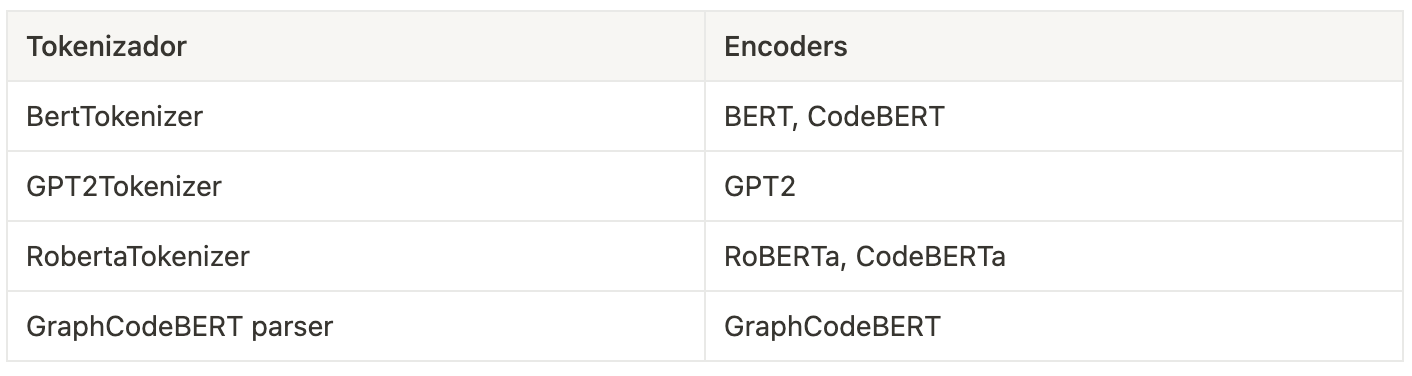
\includegraphics[scale=0.5]{tokenizers.png}
        \smallcaption{Fonte: Autor}
        \label{fig:metodology-tokenizers}
\end{figure}

\section{\textit{Encoders}}
\label{sec:methodology:encoders}
Os \textit{encoders}, relacionados na figura \ref{fig:metodology-tokenizers}, receberão os dados pré-processados para gerar os \textit{embeddings} correspondentes. Com isso, a partir dos pares código-fonte/descrição, essa etapa irá gerar pares de \textit{embeddings} código-fonte/descrição.

\section{Concatenação dos \textit{embeddings}} 
\label{sec:methodology:embeddings-concat}
Com os pares de \textit{embeddings} código-fonte/descrição gerados, esta etapa será responsável por concatenar os \textit{embeddings} contidos nesses pares. 
A concatenação desses dois \textit{embeddings} se dará juntando os dois vetores em um só, de forma que dado o primeiro vetor tenha tamanho $m$ e o segundo $n$, o tamanho do vetor resultante após a concatenação será $m + n$.
O \textit{embedding} concatenado resultante servirá como entrada para o modelo de comparação de \textit{embeddings}, descrito a seguir.

\section{Modelo de comparação de \textit{embeddings}}
\label{sec:methodology:embedding-comparator}
O modelo de comparação de \textit{embeddings} consiste em uma rede neural que, a partir de dois \textit{embeddings} concatenados, tem como objetivo determinar a similaridade entre estes dois \textit{embeddings}. A figura \ref{fig:metodology-embeddings_comparator} mostra o diagrama do modelo em questão.

\begin{figure}[htbp]
    \centering
        \caption{Comparador de \textit{embeddings}}
        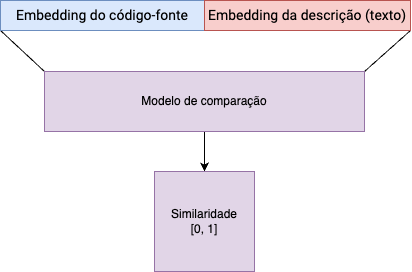
\includegraphics[scale=0.6]{emb-comparator.png}
        \smallcaption{Fonte: Autor}
        \label{fig:metodology-embeddings_comparator}
\end{figure}

Conforme apresentado no diagrama, o comparador consiste em uma rede neural, com $n$ camadas e uma função de ativação. Essa rede receberá como entrada os \textit{embeddings} do código-fonte e de sua descrição, concatenados. A saída será um valor, entre 0 e 1, que representará a similaridade entre os dois \textit{embeddings} da entrada. Tanto a topologia, quanto o número de camadas e a função de ativação serão determinados experimentalmente, conforme descrito no capítulo \ref{chp:experiments}.

\section{Etapa de inferência}
Por fim, após a etapa de treinamento do modelo de comparação de \textit{embeddings}, será realizada a etapa de inferência. Conforme descrito na figura \ref{fig:metodology-system_overview}, cada texto da base de validação será comparado com todos os códigos-fonte da mesma base, a fim de gerar um \textit{ranking} de similaridade dos códigos-fonte com o texto em questão. Esse texto representa uma consulta feita pelo usuário, em linguagem natural, ao procurar por determinado código-fonte.
Essa etapa de inferência servirá para validar o modelo de comparação. Os resultados obtidos a partir dessa etapa serão estudados de acordo com o capítulo \ref{chp:experiments}.


